\chapter{Introduction}
\begin{refsection}
\section{The great success of molecular biology}
\noindent For most of human history, the microbial world was limited to speculation and imagination.. That was until the late 17th century, when Antonie van Leeuwenhoek, a Dutch microscopist, was the first person to see microbes due to his exceptional skill in making single-lens microscopes~\citep{van1665observations,asimov1972asimov,lane2015unseen}. But it wasn't until the 19th century that Christian Gottfried Ehrenberg coined the word \textit{Bacterium} in 1828~\citep{ehrenberg1828symbolae} and Louis Pasteur disproved the theory of spontaneous generation~\citep{pasteur1862memoire}, the thought that life can commonly arise from non-living matter, and the study of bacteria became of broader interest. For the last two centuries, scientists from various backgrounds have studied the smallest forms of life as we know it. In 1885, Theodor Escherich discovered the bacterium \textit{Escherichia coli}~\citep{escherich1885darmbacterien}.
Since the isolation of its K12 strain, it has become one of the best-studied model organisms to date~\citep{bachmann1972pedigrees,doi:10.1128/jb.00230-22} and one of the greatest sources of groundbreaking and fundamental biological discoveries.

\indent Since the characterization of beta-D-galactosidase in 1950~\citep{lederberg1950beta}, the function of many genes in \textit{E. coli} K12 has been annotated. When its genome was fully sequenced for the first time in 1997, 4288 protein-coding open reading frames were identified~\citep{blattner1997complete} and genes were labeled by proposed function. Genes for which no function could be proposed either by previous work or by homology to genes with known function in other organisms were labeled with a \textit{y} as the first letter. The knowledge base of gene function in \textit{E. coli} has come so far, that it has become possible to simulate whole cell models of \textit{E. coli} cells and predict the abundance of a vast set of proteins and growth rates in a limited number of environmental conditions~\citep{sun2021coli}. The success of these predictive models relies on the fact that gene expression is not a stochastic free-for-all, but a tightly orchestrated process governed by specific regulatory logic.
%However, after 75 years of work, about one-third of \textit{E. coli}'s protein-coding sequences remain without functional annotation, a group of genes that has been coined the \textit{y-ome}~\citep{ghatak2019ome,moore2024revisiting}. In a 2016 study, the concentration of all proteins in \textit{E. coli} cells was measured in 22 different growth conditions. While the resulting data set is incredibly rich and powerful, it also shows that only about 58\% of genes account for more than 95\% of the protein mass in a cell.
\begin{figure}[hbt!]
\centering
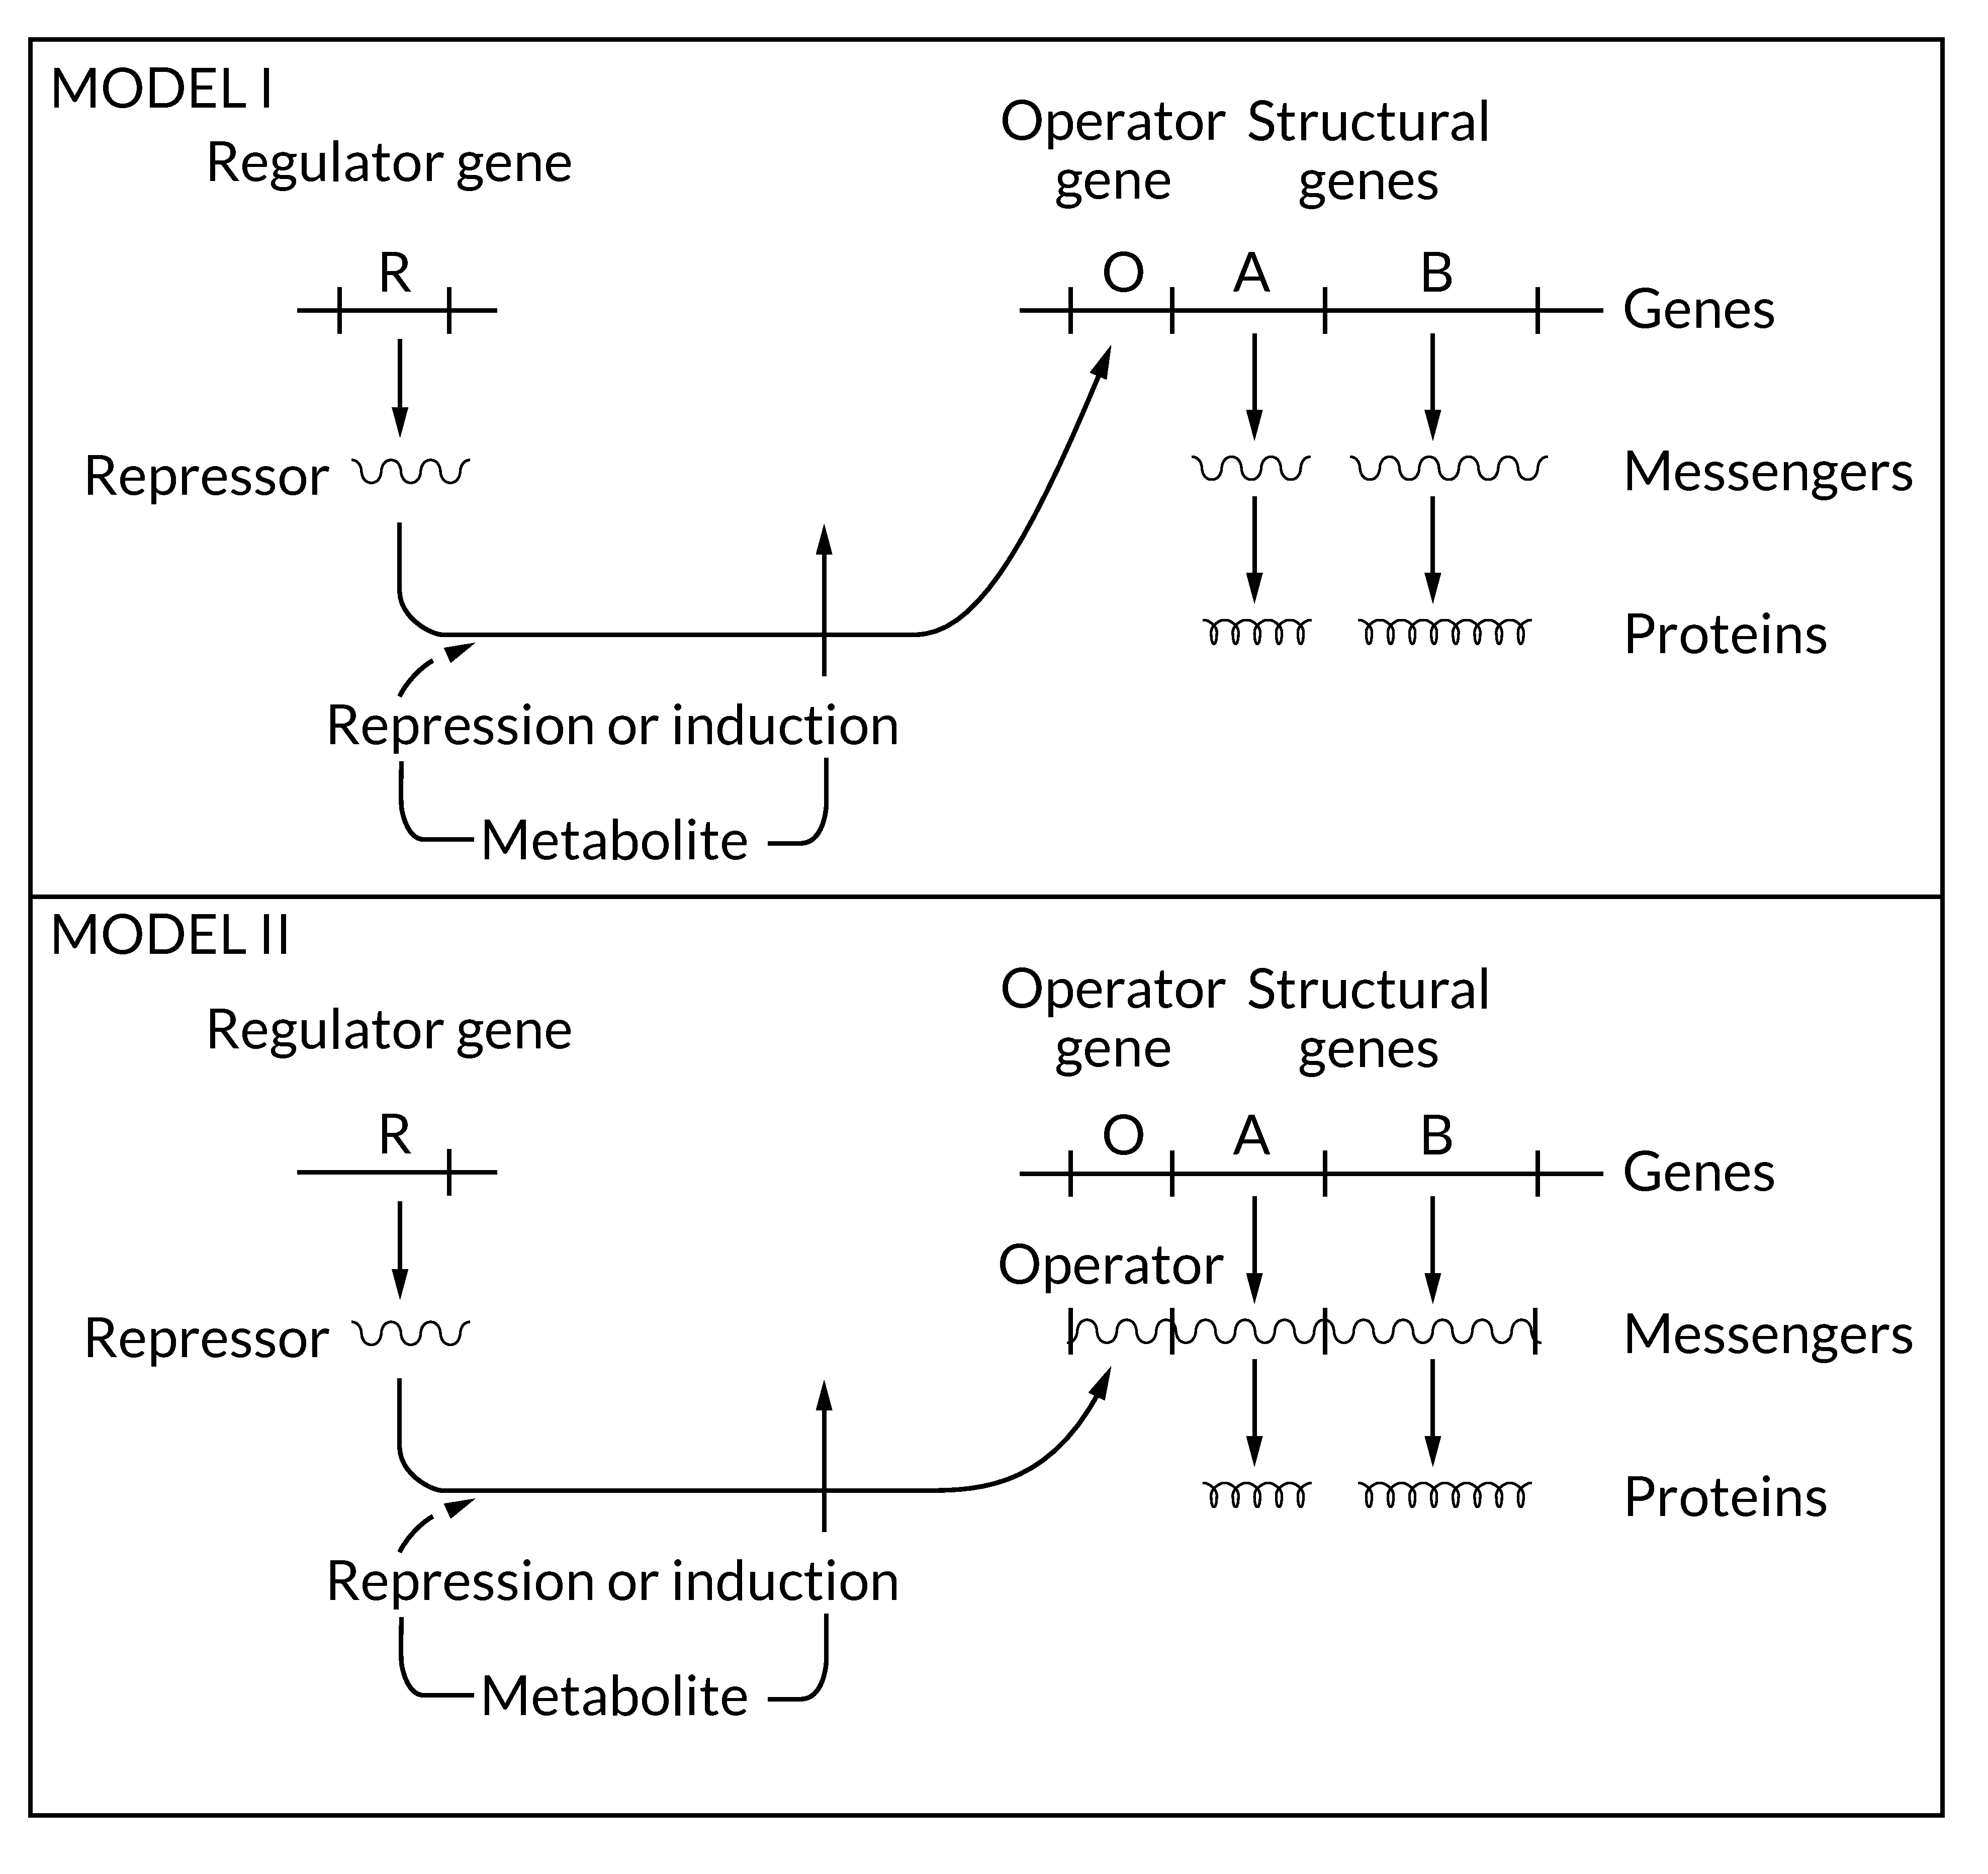
\includegraphics[width=.7\textwidth]{figures/intro/Jacob_Monod_fig6.pdf}
\caption[Discovery of gene regulation by Jacob and Monod.]{\textbf{Historical models of gene regulation in the lac operon.} Schematic representation of the two competing hypotheses proposed by Jacob and Monod: (Model 1) the genetic operator model, where the repressor acts directly on the DNA to inhibit transcription; and (Model 2) the cytoplasmic operator model, where regulation occurs at the level of the messenger RNA (translation). Kinetic evidence regarding mRNA stability ultimately favored Model 1. Adapted from \cite{jacob1961genetic}.}\label{fig:jacob_monod}
\index{figures}
\end{figure}\\
\indent In addition to identifying a gene's function, it is equally important to know when the gene is expressed. Fran{\c{c}}ois Jacob and Jacques Monod famously discovered the mechanism of repression and inducible expression of the lac-operon in 1961~\citep{jacob1961genetic}. While this work contains many more fundamental discoveries, such as the prediction of mRNA and its short lifetime and the refutation of the \textit{one gene, one enzyme} hypothesis, we focus on the discovery of the \textit{operon}. They found that a protein encoded in a different genomic location can control the expression of a set of genes by interacting with a piece of DNA. As shown in Figure~\ref{fig:jacob_monod}, Jacob and Monod discussed two possible models of repression, which they coined the "genetic operator model" (Model 1) and the "cytoplasmic operator model" (Model 2). In the genetic operator model, the repressor-operator interaction occurs at the genetic level, with the repressor directly controlling the synthesis of the gene. By considering the kinetics implied from this model, that the lifetime of the messenger molecule is short and that synthesis of the gene product should be stopped immediately once the gene is removed from the cell, this model was identified as the most likely. And as we now know, the lac repressor binds to DNA, inhibiting expression from the promoter of the lac operon by both sterically blocking binding of the RNA polymerase and by DNA looping~\citep{oehler1990three,becker2013mechanism}, and the lifetimes of mRNA are on the order of minutes~\citep{bernstein2002global}. \\
In the cytoplasmic operator model, the repressor binds to the messenger RNA, regulating its translation into protein. Jacob and Monod conclude that this model is unlikely because the size of RNA molecules it would require does not agree with the distributions of mRNA sizes measured at the time. Also, this model would require the messenger molecule to have much longer lifetimes. Jacob and Monod specifically noted that they could not disprove this model, and now we know that parts of it exist as small RNAs that can inhibit translation of mRNAs~\citep{masse2002small}. It should also be noted that at the time of this work, the details of the transcritption-translation machinery were still getting figured out, which makes the discoveries and predictions Jacob and Monod proposed even more impressive.\\
\indent While Jacob and Monod established the fundamental logic of genetic switches, their work primarily focused on the existence of these regulatory interactions. In the decades that followed, the field shifted from identifying these "logic gates" to uncovering the precise molecular architectures that govern them. This transition revealed that regulation is often far more structurally complex than simple steric hindrance. As we will see, moving from a qualitative understanding to a predictive, quantitative theory requires both a detailed map of molecular geometry—such as that found in the \textit{ara} operon—and a physical framework to translate those geometries into mathematical functions. As will be explained below, it is fair to say that we both know a lot and at the same time very little about how genes are regulated in bacteria.
\begin{figure}[hbt!]
\centering
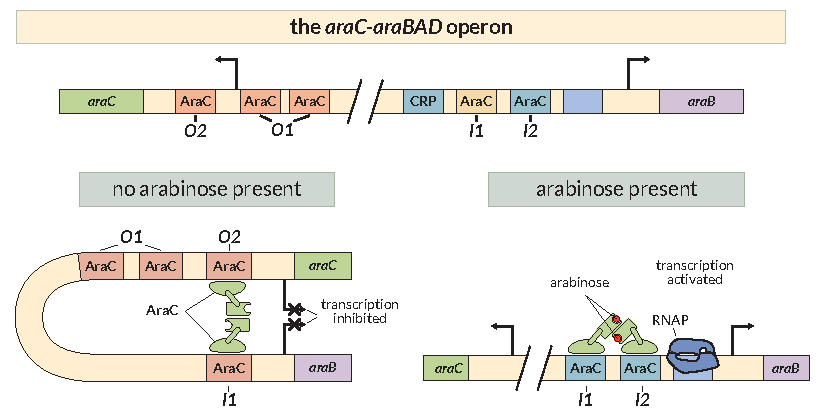
\includegraphics[width=\textwidth]{figures/intro/araB_operon_annotation.pdf}
\caption[Regulatory architecture of the araBAD operon.]{\textbf{Regulatory architecture of the araBAD operon.} (Left) In the absence of L-arabinose, the AraC homodimer binds to the distal \textit{I1} and \textit{O2} sites, forming a DNA loop that sterically hinders RNA polymerase binding at the.  Adapted from \cite{schleif2010arac}}\label{fig:araBAD}
\index{figures}
\end{figure}
\\ 
\indent One of the best studied operons in \textit{E. coli} is the \textit{ara}-operon, which was investigated in rigorous detail by the lab of Robert Schleif. This operon is responsible for the metabolism of L-arabinose and consists of the genes \textit{araBAD} and its divergently expressed regulator \textit{araC}~\citep{greenblatt1971arabinose}. As shown in Figure~\ref{fig:araBAD}, it was discovered that in the absence of L-arabinose, AraC forms a tetramer and binds to two distant binding sites (\textit{I1} and \textit{O2}), leading to the formation of a DNA loop, which suppresses expression from the promoters for \textit{araC} and \textit{araBAD}~\citep{dunn1984operator,martin1986dna,lobell1990dna}. If L-arabinose is present, it binds to each AraC dimer, leading to a conformational change and binding of the complex to the \textit{I1} and \textit{I2} binding sites in the \textit{araBAD} promoter. In this configuration, AraC initiates transcription, and arabinose is metabolised~\citep{schleif2010arac}.

\indent In addition to having a detailed understanding of molecular mechanisms for certain promoters, we have quantitative input-output functions for gene expression of promoters given variations in a diverse range of biophysical parameters. DNA-binding proteins often recognize specific DNA sequences as targets for binding, and the binding affinity is specific to those sequences. Using thermodynamic models, this binding affinity is quantified as binding energy. In the case of transcription factors, such thermodynamic models can be used to predict relative changes in gene expression, often expressed as fold changes. The key quantity in such models is the partition function — the sum of the statistical weights of all possible states. Each state is defined by a weight, which contains the parameters of interest. The probability of a certain state being occupied is then given by the ratio of the weight to the partition function. Predictions of gene expression values are given by the probability of RNA polymerase binding to DNA~\citep{ackers1982quantitative,shea1985or,record1996escherichia}.

\indent A well-studied example is the lac repressor, LacI, in \textit{E. coli}, which represses the lac operon in the absence of allolactose by DNA looping (similar to AraC described above). There are three binding sites for LacI in the \textit{E. coli} genome, lac\textit{O1}, lac\textit{O2} and lac\textit{O3}~\citep{oehler1990three}. For each of these binding sites, and an additional binding site which is predicted to be the strongest binding site for LacI possible, lac\textit{Oid}, affinities were experimentally derived and used to predict fold-change for varying numbers of LacI proteins in the cell~\citep{garcia2011quantitative}. The binding affinities are usually given in units of $k_BT$ relative to binding to a random DNA sequence, which is called non-specific binding~\citep{von1986specificity}. 

\indent While the occupancy of these repressor sites sets the stage for regulation, the model equally depends on the recruitment of the transcription machinery itself. The state that leads to expression from the promoter depends on the binding affinity of RNAP (including sigma factors in these models). The stronger the binding affinity, the more likely the RNAP-bound state is, which is the transcriptionally active state~\citep{mcclure1985mechanism}. In previous work, the binding affinity of multiple variants of the promoter of the lac operon was determined via three distinct methodologies: SORT-Seq (discussed in Section~\ref{sec:binding_sites})~\citep{kinney2010using}, enzymatic assays, and single-cell mRNA FISH~\citep{brewster2012tuning}. There was good agreement between the results, showing the robustness of the model and the parameters to the experiments from which they were derived. 

\indent These individual binding affinities, however, do not exist in isolation; the global availability of transcription factors is often constrained by the total number of binding sites across the genome. There can be multiple binding sites for transcription factors in a cell, either because there are multiple binding sites in the genome or because reporters are delivered on plasmids with varying copy numbers. Titration becomes critical when the copy number of the transcription factor is lower than or of the same order of magnitude as the number of binding sites in the cell. In that scenario, the number of available transcription factors that can bind each site is effectively reduced because transcription factors are already bound to other sites~\citep{buchler2003schemes}. This titration effect can also be quantitatively described by thermodynamic models even when the sites have varying binding affinities~\citep{gerland2002physical,rydenfelt2014statistical,brewster2014transcription}.

\indent Beyond the simple availability of proteins, the spatial arrangement of these binding sites can introduce more complex regulatory architectures, most notably through DNA looping, where a transcription factor, usually as a homotetramer, binds in two distant sites. This brings these two regions into close physical proximity, forming a DNA loop that makes the region inaccessible to transcription. Extensive studies have applied statistical mechanics to DNA looping using tethered particle motion, including parameters such as the concentration of the transcription factor~\citep{johnson2012sequence}, the binding affinities of each binding site~\citep{johnson2012sequence}, and the length of the DNA spacer between the binding sites~\citep{han2009concentration,boedicker2013theoretical}. These models extend the predictive power of thermodynamics to more complex mechanisms of gene regulation~\citep{vilar2003dna,vilar2005dna,saiz2007multilevel,saiz2008ab}.

\indent These structural models provide a framework for repression, yet the system must also remain responsive to environmental cues through allostery. Many proteins, and therefore transcription factors, are allosteric, i.e., they adopt different conformations upon binding a specific molecule. In the case of the lac repressor, in the absence of allolactose, the transcription factor takes a conformation in which it binds DNA tightly. If allolactose is present, it binds to the lac repressor, leading to a conformational change that strongly reduces its binding affinity. Input-output functions can be extended to include the inducer concentration, its binding affinity to the protein, and the change in the protein's binding affinity to DNA upon inducer binding. Experiments using IPTG, an alternative inducer of the lac repressor, show that the predictive power of thermodynamic models extends well into the induction regime~\citep{razo2018tuning}. Allostery also enables finetuning of entire genetic circuits, such as the bistable switches or genetic oscillators~\citep{elowitz2000synthetic,gardner2000construction,yang2025dynamics}.

\indent While these models describe how environmental signals modulate protein activity, they also allow us to predict how the underlying DNA sequence dictates the baseline affinity of the system. This introduces the question of how the transcription factor's binding affinity is modified when the DNA sequence is mutated at any position. This has been a topic of research for many decades, and in many theoretical models, a generic energy cost was associated with mutations~\citep{berg1987selection,stormo1998specificity,lassig2007biophysics}. However, we can do better than generic energy costs and determine the cost of each mutation in high-throughput mutagenesis experiments. The result is an energy matrix that provides precise energy costs for each possible mutation from a reference sequence, as in the case of the lac repressor binding sites~\citep{barnes2019mapping}. Such models assume that if multiple mutations occur, their separate effects on the binding affinity are additive, an assumption that holds well for up to four mutations in the lac repressor binding sites~\citep{barnes2019mapping}. 

\indent The logic of sequence-to-affinity mapping applies not only to the DNA binding sites but also to the amino acid sequence of the transcription factors themselves. Mutations in the transcription factor in its DNA binding or inducer binding regions can be accurately described by changes in the respective binding affinities and dissociation constants, maintaining the predictive power of statistical mechanics. 


\begin{figure}[hbt!]
\centering
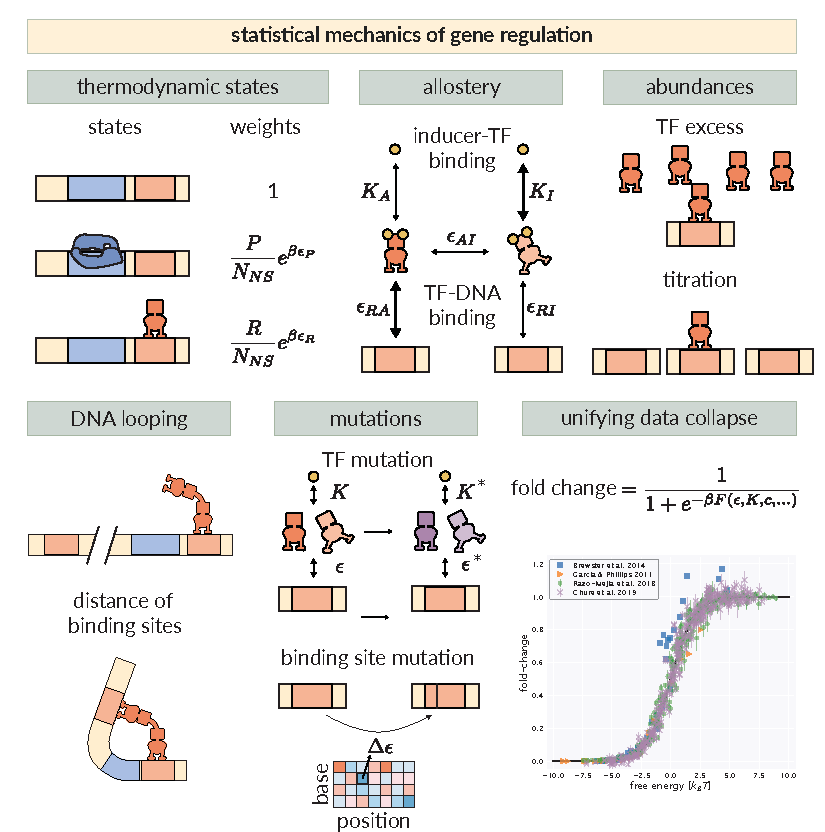
\includegraphics[width=\textwidth]{figures/intro/stat-mech_gene-regulation.pdf}
\caption[Statistical mechanics of gene regulation]{\textbf{Statistical mechanics of gene regulation.} Thermodynamic states are quantified by their Boltzmann weights. Transcription factors can be allosteric, where the inducer molecule binds to the protein and stabilizes a non-regulating conformation. Abundances of transcription factors relative to the number of target binding sites becomes crucial when binding sites are more abundant, creating a titration effect. Distant sites can regulate transcription by forming a DNA loop when bound by a transcription factor. Mutations in the transcription factor itself can be mapped to differences in the binding affinites to DNA or inducer. One unifying free energy collapes pertubations to all these parameters to a single master curve.}
\label{fig:statmech}
\index{figures}
\end{figure}


\indent This vast set of parameters accumulates in a powerful data collapse, where data from experiments of diverse perturbations collapse on a single curve, unifying many different aspects of gene regulation into a single, predictive theory. It highlights the universality of the underlying Boltzmann distribution; whether binding affinities or copy numbers are changed, the model of gene regulation obeys the same thermodynamic master curve. The existence of such a curve demonstrates that our understanding of these systems has reached a point where we are no longer merely describing biological phenomena, but predicting them from first principles. By knowing the DNA sequence and the protein concentrations, we can accurately calculate the census of RNA polymerase on a promoter and, by extension, the physiological state of the cell.

\indent While the majority of these regulatory motifs are well-described by the "passive" occupancy models of thermodynamic equilibrium, recent work has explored how the cell adds layers of sophistication through energy-consuming processes. As shown in Figure~\ref{fig:graphs}, by allowing certain transition rates to break detailed balance—often through the hydrolysis of ATP—the cell can achieve non-monotonic dose-response curves or ultra-sensitive switches that exceed the limits of equilibrium models~\citep{mahdavi2024flexibility}. Rather than contradicting the thermodynamic framework, these non-equilibrium models represent the "fine-tuning" of an already robust system, allowing for a level of regulatory flexibility that matches the complexity of the environments in which these bacteria thrive.
\begin{figure}[hbt!]
\centering
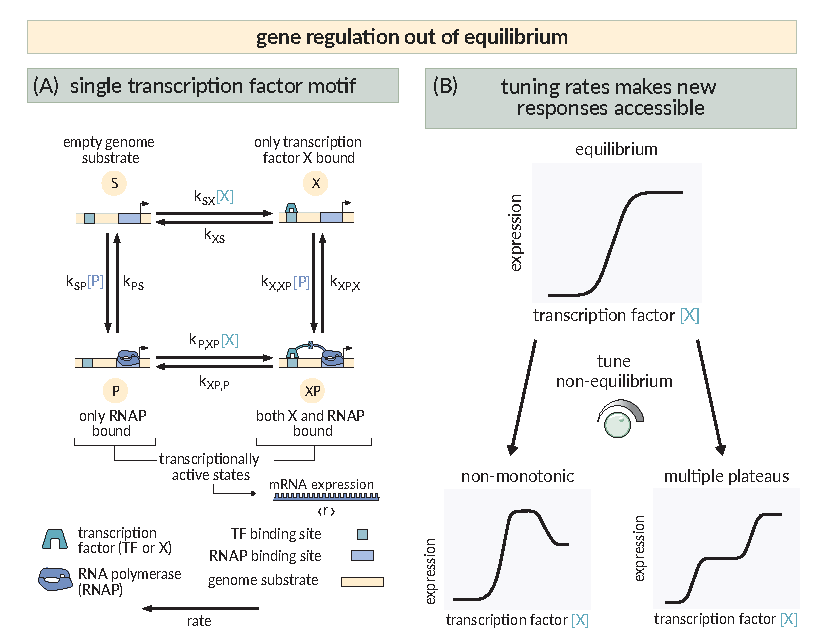
\includegraphics[width=\textwidth]{figures/intro/graphs.pdf}
\caption[graphs]{\textbf{Non-equilibrium gene regulation via graph theory.} (A) A four-state cycle representing a single transcription factor regulating a promoter. In equilibrium models, transition rates satisfy detailed balance. (B) By relaxing the equilibrium assumption and introducing energy-consuming transitions (e.g., via ATP hydrolysis), the system can achieve complex regulatory behaviors, such as intermediate plateaus or non-monotonic dose-response curves, which are inaccessible to standard thermodynamic models. Adapted from \cite{mahdavi2024flexibility}}\label{fig:graphs}
\index{figures}
\end{figure}

\indent In summary, the study of gene regulation in \textit{E. coli} has evolved from the discovery of logical switches to a comprehensive biophysical theory. We now possess a detailed map of how molecular geometry, DNA sequence, and protein-protein interactions converge to control the flow of genetic information with remarkable precision.

\section{Genomic dark matter}
\noindent Despite the remarkable success molecular biology has had, for many genes even in \textit{E. coli}, the function and transcription factors controlling their expression remain elusive. The collection of genes with little to no evidence for their function is referred to as the \textit{y-ome}, following the convention of names for genes without known function starting with y~\citep{blattner1997complete,ghatak2019ome,Moore2024_revisiting_yome}. Recent surveys of databases for \textit{E. coli} have concluded that about 35\% of genes belong to the y-ome, an astonishing number, which is also expected to be one of the limiting factors for whole cell models~\citep{sun2021coli}. Recent approaches have used artificial intelligence to predict functions from large omics datasets, showing how computational approaches can guide specific experiments more directly~\citep{Chakraborty2025_ecoli_hypothetical}. It will require a large effort to solve the remaining genes in the y-ome, specifically by expanding the realm of conditions cells are commonly exposed to in laboratory contexts.

\indent While there are many dark spots remaining in the functional landscape in \textit{E. coli}, the regulatory landscape is much dimmer in comparison. Multiple genes are often expressed on the same transcript, known as a transcription unit (TU). There are a total of 11,491 annotated transcription units in \textit{E. coli}, which is higher than the number of genes as a single gene can be in more than one transcription unit. A transcription factor often controls the expression of multiple genes at the same time by regulating the transcription unit as a whole, rather than each gene independently. Given the currently curated transcription units in RegulonDB 14, about 42\% of protein-coding genes lie in at least one transcription unit with curated TF regulation~\citep{Salgado2023RegulonDB,RegulonDB14}(\tr{add details for calculation later}). As a consequence, more than half of the genes in \textit{E. coli} have no experimentally annotated, functional transcription factor binding sites controlling their regulation. For the transcription units with curated TF regulation, there could be additional, experimentally unobserved binding sites which have not been discovered yet. Later we will discuss multiple methods that were developed in order to tackle this problem.

\section{The Era of Sequencing}
\noindent In the modern era, DNA sequencing has become a technique so ubiquitous, it has infiltrated many corners of our lives beyond the natural sciences, such as paternity and ancestry tests, and criminal investigations. Sequencing data is being generated at will in amounts that were unimaginable just two decades ago. Modern sequencers, such as the NovaSeq Series X from Illumina, can produce around 10TB of raw sequencing data a day~\citep{NovaSeqXThroughput}. If we estimate that there are around 3000 of such machines in use around the world, the total amount of data produced comes to 30PB per day. That's about $10^5$ base model iPhone 17s (256GB of storage) per day that would be required to store the data. To compare this to other big data producers in science, the largest optical observatory, the Vera C. Rubin Observatory in Chile, produces about 20TB of data per night~\citep{RubinObservatoryData}. There are only a handful of optical observatories around that produce such amounts of data, so it does not come close to the amount of sequencing data produced. Larger producers of data are coming from radio astrometry, like the Square Kilometre Array, which is producing hundreds of petabytes per year, i.e., hundreds of TB of retained data per day~\citep{SKADataVolume}. We can estimate there to be around 10 of such facilities of equal or less data production around, leading to an upper bound of a few petabytes per day of retained data production, which is still less than the estimated amount of produced sequencing data. These rough estimates underscore that biological data generation has reached unprecedented scales, while our ability to uniformly process, interpret, and integrate these data lags far behind.

\indent Genomic science was already an intense field of research even before DNA sequencing was available. In the late 1940s, Linus Pauling proposed that hereditary diseases could be caused by a specific molecular variant of a protein. He studied hemoglobin and its properties in patients with sickle cell anemia, a disease in which red blood cells become distorted at low oxygen levels, leading to multiple symptoms, including blockage of small blood vessels. In his research, he studied hemoglobin extracted from healthy individuals and compared it with hemoglobin from individuals diagnosed with the disease. Both proteins were run in a moving-boundary electrophoresis experiment, where molecules separate by charge~\citep{Tiselius1937Electrophoresis}. He found that the hemoglobin extracted from patients with the disease moved differently from that extracted from healthy individuals. The two species of hemoglobin were clearly distinguishable. A third sample from patients with a less severe type of the disease, sicklemia, had a mixture of the two species~\citep{Pauling1949SickleCell}. 

\indent Inspired by Pauling's results, Vernon Ingram studied the same proteins using a peptide fingerprinting technique, in which proteins are digested with the protease trypsin, yielding multiple smaller peptide chains. The peptide chains are then run on a two-dimensional assay, where peptides are separated by charge on one axis and hydrophobicity on the other. Ingram found that the two hemoglobin species were mostly the same, up to one spot that was more positively charged in the sick species than the corresponding spot in the healthy one~\citep{Ingram1956Hemoglobin}. At this point in time, due to Frederick Sanger's work on Insulin~\citep{sanger1952arrangement}, it was established that proteins were amino acid sequences, and the first methods of reading protein sequences were available. Shortly after Ingram's discoveries, he identified the peptide sequence that differed between the two hemoglobin species and found that only a single amino acid was different: glutamic acid was mutated to valine, which removed a negative charge from the peptide. This was the first time a human disease was attributed to a single amino acid substitution.

\indent It wasn't until twenty years after Ingram's discovery that the first DNA sequencing method became available. At this point, the genetic code had been solved, but reading DNA sequences was still not readily accessible. In 1977, Frederick Sanger developed a chain-termination method to obtain DNA sequences. Single-strand DNA templates are copied using supplemented nucleotides. The ingenuity was to add dideoxynucleotides, which terminate DNA polymerase replication, thereby stopping the replication process. Sanger performed four separate experiments, in each of which one dd-nucleotide species was added to a mix of the four regular nucleotides. This leads to termination of replication for a subset of DNA strands every time the letter of the corresponding dd-nucleotide is added. DNA molecules are separated by length by a denaturing polyacrylamide gel. For each reaction, this yields a ladder of bands, where each band indicates a DNA fragments that were elongated to a specific position. Since only one dd-nucleotide was added per reaction, each band in the ladder corresponds to reading this specific nucleotide at that position~\citep{sanger1977dna}. 

\indent One of the limiting factors to DNA sequencing was the amount of template that was needed, limiting its application to a few use cases. This changed dramatically with the invention of polymerase chain reactions (PCRs) in 1983 by Kary Mullis, which is arguably the most groundbreaking and widely used technique in molecular biology today~\citep{mullis198721}. PCR allows the exponential amplification of DNA, which enables the creation of large amounts of DNA from very small template amounts. Using PCR, DNA sequencing became much more accessible to more applications. However, still only one relatively short DNA template (on the order of hundreds of base pairs) can be sequenced by Sanger sequencing at the same time, limiting the throughput. Yet, the immense success of DNA sequencing in the following years is undeniable. As we discussed above, in 1997 the first complete genome of \textit{E. coli} K12 was obtained, followed by the first human genome in 2001~\citep{international2001initial}. For both these discoveries, Sanger sequencing was used to obtain the sequences.

\begin{figure}[hbt!]
\centering
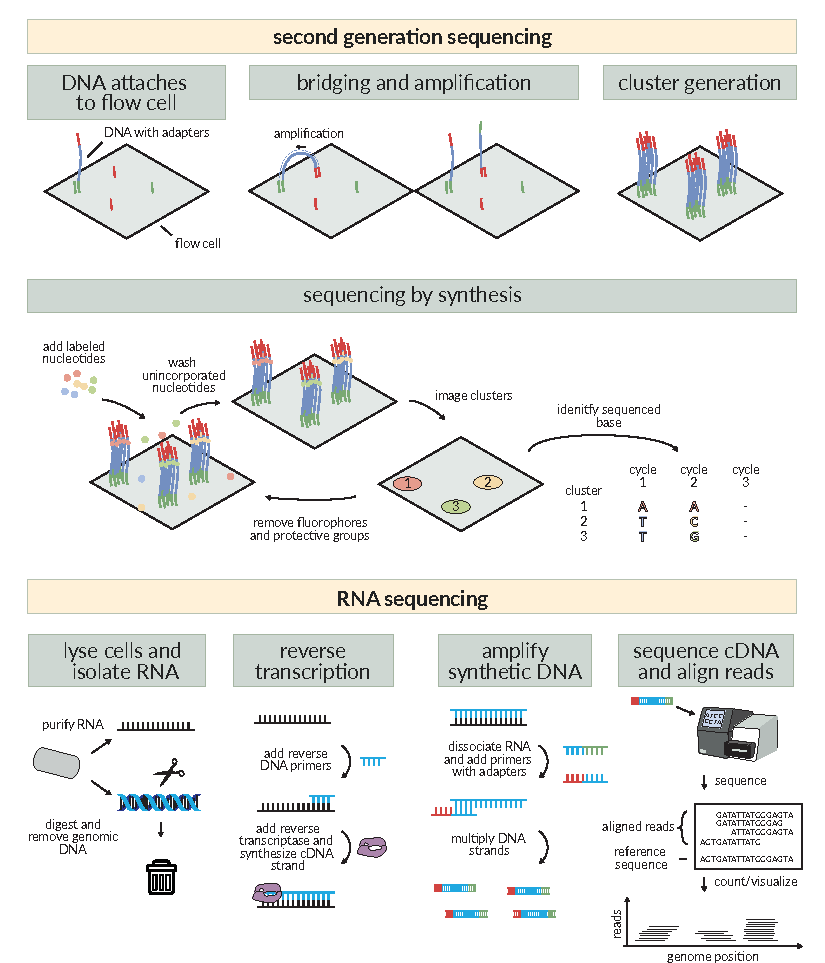
\includegraphics[width=\textwidth]{figures/intro/ngs_method.pdf}
\caption[Second generation sequencing and RNA-Seq]{\textbf{}}\label{fig:sequencing_backgrounds}
\index{figures}
\end{figure}

\indent The problem of scaling sequencing was tackled soon after, with the introduction of the first Next-Gen-Sequencing (NGS) technologies. The most commonly used technology was developed by Solexa, later acquired by Illumina, and uses sequencing by synthesis. The basis is a flow cell containing many short DNA oligonucleotides that allow DNA templates containing the complementary sequence, called adapters, to stick to the flow cell. The key is that there are two adapter sequences, one on each side of the DNA sequence, which allow the sequence to form a bridge, enabling bridge amplification and the formation of clonal clusters. After DNA sequences are amplified and clusters are formed, DNA sequences are synthesized one base at a time, and fluorophore-tagged nucleotides are used. After each step in the synthesis, fluorescent imaging is performed on the clusters, and the nucleotide is identified by the tagged fluorophore. Since each cluster is read separately, they don't need to contain the same sequence, which makes it possible to sequence many sequences at the same time. This decouples sequencing throughput from fragment identity~\citep{bentley2008accurate}. 

\indent With Next-Gen-Sequencing, DNA could be read massively in parallel and throughput became much less limiting. This led to the exploration of new realms in biology, with one path going beyond just reading DNA, but moving towards its interpretation, completely revolutionizing the study of the transcriptome. A crucial component was the reverse transcriptase, discovered in the 1970s~\citep{temin_viral_1970,baltimore1970viral}. This enzyme can translate RNA into DNA, against the direction of the central dogma. In a series of landmark studies, it was shown how cellular RNA is reverse transcribed into synthetic DNA (called cDNA), which then can be sequenced by NGS. Relative abundances of cDNA can be interpreted as differences in abundances of the underlying RNA, giving a measure of gene expression across the entire cell~\citep{mortazavi2008mapping,nagalakshmi2008transcriptional}. A vast array of X-seq methods were developed since then, covering vastly different scientific questions, such as defining cell types by which transcripts they express, which led to the creation of the human cell atlas, a map of every cell in the human body~\citep{regev2017human}. Because transcription factors ultimately exert their effects through changes in RNA abundance, RNA sequencing provides a direct and quantitative readout of regulatory activity across the genome. Other methods use RNA-Seq to discover binding sites for transcription factors in prokaryotes, such as Reg-Seq, which is the foundational method of this paper and will be discussed in detail.


\section{Discovery of DNA binding sites}
\label{sec:binding_sites}
\noindent Jacob and Monod hypothesized that a protein binds to DNA to control expression from the \textit{lac}-operon, but the direct interaction was not experimentally proven yet. Walter Gilbert and Benno M\"uller-Hill figured out that the lac repressor physically binds to DNA, and that the binding is specific to a region in the \textit{lac}-operon, and that the lac repressor does not bind any other DNA~\citep{gilbert1967lac}. Around the same time, Mark Ptashne made similar observations for the $\lambda$ repressor~\citep{ptashne1967specific}. These fundamental findings brought experimental evidence that transcription factors bind specific DNA regions. These regions were not very precise yet, until Walter Gilbert and Allan Maxam first used a DNase assay to identify the sequence of the operator~\citep{gilbert1973nucleotide}. Protein and DNA are incubated such that the protein binds to its specific binding sites. Then, a deoxyribonuclease is used to digest DNA that is not bound by protein, leaving only the protected DNA, for which the DNA sequence was identified.


\indent This concept was then translated into a general method to identify the sequences for DNA binding proteins, DNAse footprinting~\citep{galas1978dnaase}. A candidate DNA sequence is needed in advance, such it can then be narrowed down using the assay. For a while, this was the established method to localize DNA binding sites. But it was hard to identify binding sites for a DNA binding protein if there was no candidate DNA to begin with. This was addressed a method called systematic evolution of ligands by exponential enrichment (SELEX), which was initally developed for RNA~\citep{TuerkGold1990}, and shortly thereafter for DNA as well~\citep{blackwell1990differences}. In SELEX, a pool of synthetic oligonucleotides is incubated with the target protein. Unbound sequences are washed away, and bound sequences are amplified. This step is repeated for several iterations, continuously enriching for the strongest binding sequences. More recently, SELEX has been deployed to generate a large database of binding sequences for many transcription factors in \textit{E. coli}~\citep{ishihama2016transcription}.

\indent The need for multiple iterations is removed by the use of protein-binding microarrays (PBM)~\citep{bulyk2001exploring}. A microarray is equipped with a vast array of different DNA sequences, and the protein of interest is incubated with the DNA in each well. The protein is tagged with a fluorophore, and after unbound protein is washed away, fluorescence is measured in each well. The amount of fluoresence correlates with the amount of protein bound to the DNA specific to the well, giving a readout about with DNA sequence the protein binds tighter to. The design of the microarrays was further improved to include all k-mers of length ten, vastly exploring sequence space~\citep{berger2006compact}. While this exploration is very extensive, the DNA is immobilized in the array and proteins have to be tagged for fluoresence. Another approach is to use genomic DNA as template for \textit{in vitro} assays, limiting the possible sequence space to a more informed subset~\citep{OMalley2016}. Proteins are bound to beads, immobilzing it instead of the DNA. Similar to SELEX, DNA bound to protein is purified, but instead of iterative enrichment, only one round of binding is performed. 

\indent One common thread of all methods mentioned beforehand is that protein--DNA binding is probed \textit{in vitro}. While this allows for reproducible conditions, it ignores aspects of the cellular context that can be essential for regulatory interactions. For example, many transcription factors are allosterically regulated or undergo post-translational modification in response to environmental cues. A prominent example is the cAMP receptor protein (CRP) in \textit{E. coli}, whose DNA-binding activity depends on binding of the effector molecule cAMP~\citep{majors1975specific}, and whose stable occupancy and transcriptional activation at many promoters are further mediated by cooperative interactions with RNA polymerase~\citep{busby1999transcription}. This context dependence complicates the direct extrapolation of \textit{in vitro} binding measurements to regulatory behavior in vivo. 

\indent Measurements of DNA-protein binding inside the cell are difficult, as such interactions are usually disrupted when cells are lysed. One way to circumvent this issue is to crosslink contacts between proteins and DNA (and other proteins associated with DNA such as histones) using formaldehyde, creating covalent bonds. This stabilizes the complex, and allows for purification of specific proteins and extraction of the DNA associated with them. This method was already used in the 80s to study the heat shock response in \textit{D. melanogaster}~\citep{solomon1988mapping}. Later, the method was combined with DNA microarrays to identify the sequences that were retrieved, allowing idendentification of the target sequence without DNA sequencing~\citep{ren2000genome}. After the development of next-gen-sequencing, it became possible to identify DNA sequences bound to protein without having to design microarrays in advance. Using ChIP-Seq, DNA sequences are identified by sequencing, and then mapped onto a known genomic sequence to idenity where in the genome binding occurs, enabling whole genome scans~\citep{Johnson2007}. Since its development, ChIP-Seq has been further improved to increase the resolution of identified binding sites by the use of exonucleases that chew away unprotected DNA before DNA is eluted from protein~\citep{rhee2011comprehensive}.

\indent ChIP-Seq has been used to great success to identify DNA binding sites in plenty of different organisms. But more recently, it has been shown that DNA binding does not strictly correlate with function. In the case of \textit{E. coli} PhoB, some intergenic and most intragenic binding sites identified by ChIP-Seq did not affect expression of any gene when bound by PhoB~\citep{fitzgerald2023genome}. This points to a more general conundrum all previously discussed methods of binding site identification have: binding of a transcription factor alone is not indicative of transcriptional regulation. Functional readouts require another step to verify changes in transcription levels upon binding of the transcription factor. In the context of DNase footprinting assays, this has been accomplished by combining the readout of protein occupancy on the genome with RNA polymerase ChIP-Seq measurements, as RNA polymerase occupancy is a procy for transcription rates~\citep{trouillon2023genomic}.

\begin{figure}[hbt!]
\centering
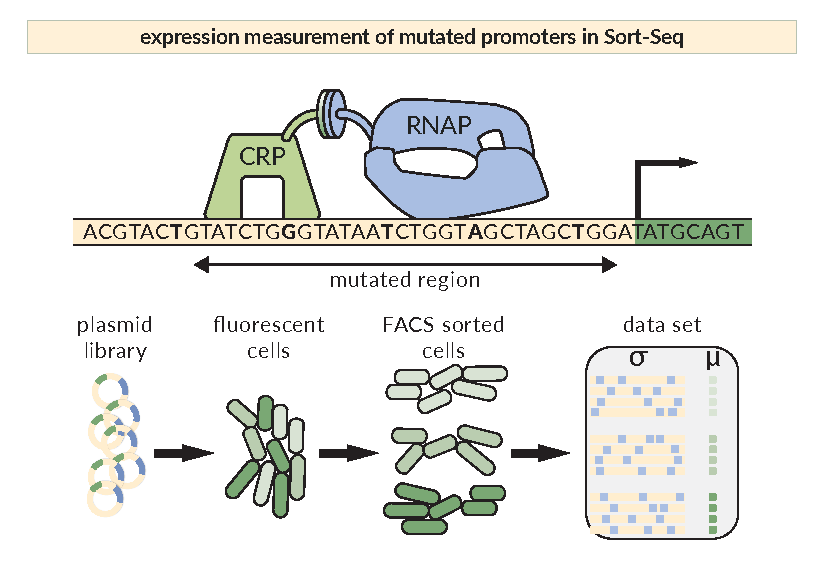
\includegraphics[width=\textwidth]{figures/intro/sort-seq_experiment.pdf}
\caption[Sort-Seq experiment]{\textbf{S.} Adapted from~\cite{Kinney2010}}\label{fig:sort-seq}
\index{figures}
\end{figure}

\indent A direct way to identify functional binding sites for transcription factors is by mutagenesis for promoter regions. In 2010, Justin Kinney et al. developed Sort-Seq~\citep{Kinney2010}. As has been discussed above, binding of a transcription factor is specific to the sequence of its binding site, and mutations in the binding site can reduce binding affinity and therefore its effect on transcription rates. By cloning randomly mutated promoter variants upstream of a fluorescent reporter gene, measured fluorescence can be correlated with the location of mutations and binding sites can be identified. As a way to increase the throughput of measurements, cells were sorted using fluorescent activated cell sorting (FACS), which splits the cells into different pools given their observed levels of fluoresence. Each pool is then sequenced using NGS, leading to a direct connection between the sequence and its mutations, and the resulting change in expression. As proof of concept, the binding site for CRP was idenitfied together with the binding of RNAP through $\sigma_{70}$. This method was then used to discover new binding sites in three different promoters, highlighting the potential as a discovery tool~\citep{Belliveau2018}. The identity of the transcription factor was then identified by DNA chromatography and mass spectrometry, which will be discussed more in detail below.

\section{Deciphering regulatory architectures in high-throughput}
In the previous sections we have discussed the rise of DNA and RNA sequencing as everyday tools, as well as mutagenesis based approaches to identifying regulatory binding sites. These two paths meet in a method called Reg-Seq. The details of the method will be discussed below, but I want to give a brief overview to motivate the approach. As basis for promoter mutagenesis, a region of 160 base pairs around the transcription start site is chosen, from 115 bases upstream of the transcription start site to 44 bases downstream. While the total length of the promoter region is limited by the cost and length limitations of commercial oligo synthesis, most known transcription factor binding sites are within this region \tr{working on a figure for this}. However, this biases the region in which we can make new discoveries, and in later chapters we will discuss how the experiment could be changed in the future to address this issue.



\begin{itemize}
    \item gel mobility assay 
    \item  
\end{itemize}
\section{Description of chapters}
\begin{itemize}
    \item HERNAN seq
    \item Description of Reg-Seq experiment and summary statistics
    \item Data Processing of Reg-Seq
    \item binding sites
    \item De novo promoters
    \item other interesting results
    \item Future experiments
    \item 
    \item 
\end{itemize}

\printbibliography[heading=subbibliography]
\end{refsection}